%%%%%%%%%%%%%%%%%%%%%%%%%%%%%%%%%%%%%%%%%%%%%%%%%%%%%%%%%%%%%%%%%%%%%%
%%  Copyright by Wenliang Du.                                       %%
%%  This work is licensed under the Creative Commons                %%
%%  Attribution-NonCommercial-ShareAlike 4.0 International License. %%
%%  To view a copy of this license, visit                           %%
%%  http://creativecommons.org/licenses/by-nc-sa/4.0/.              %%
%%%%%%%%%%%%%%%%%%%%%%%%%%%%%%%%%%%%%%%%%%%%%%%%%%%%%%%%%%%%%%%%%%%%%%


\newcommand{\commonfolder}{../../common-files}

\documentclass[11pt]{article}

\usepackage[most]{tcolorbox}
\usepackage{times}
\usepackage{epsf}
\usepackage{epsfig}
\usepackage{amsmath, alltt, amssymb, xspace}
\usepackage{wrapfig}
\usepackage{fancyhdr}
\usepackage{url}
\usepackage{verbatim}
\usepackage{fancyvrb}
\usepackage{adjustbox}
\usepackage{listings}
\usepackage{color}
\usepackage{subfigure}
\usepackage{cite}
\usepackage{sidecap}
\usepackage{pifont}
\usepackage{mdframed}
\usepackage{textcomp}
\usepackage{enumitem}
\usepackage{ctex}


% Horizontal alignment
\topmargin      -0.50in  % distance to headers
\oddsidemargin  0.0in
\evensidemargin 0.0in
\textwidth      6.5in
\textheight     8.9in 

\newcommand{\todo}[1]{
\vspace{0.1in}
\fbox{\parbox{6in}{TODO: #1}}
\vspace{0.1in}
}


\newcommand{\unix}{{\tt Unix}\xspace}
\newcommand{\linux}{{\tt Linux}\xspace}
\newcommand{\minix}{{\tt Minix}\xspace}
\newcommand{\ubuntu}{{\tt Ubuntu}\xspace}
\newcommand{\setuid}{{\tt Set-UID}\xspace}
\newcommand{\openssl} {\texttt{openssl}}


\pagestyle{fancy}
\lhead{\bfseries SEED Labs}
\chead{}
\rhead{\small \thepage}
\lfoot{}
\cfoot{}
\rfoot{}


\definecolor{dkgreen}{rgb}{0,0.6,0}
\definecolor{gray}{rgb}{0.5,0.5,0.5}
\definecolor{mauve}{rgb}{0.58,0,0.82}
\definecolor{lightgray}{gray}{0.90}


\lstset{%
  frame=none,
  language=,
  backgroundcolor=\color{lightgray},
  aboveskip=3mm,
  belowskip=3mm,
  showstringspaces=false,
%  columns=flexible,
  basicstyle={\small\ttfamily},
  numbers=none,
  numberstyle=\tiny\color{gray},
  keywordstyle=\color{blue},
  commentstyle=\color{dkgreen},
  stringstyle=\color{mauve},
  breaklines=true,
  breakatwhitespace=true,
  tabsize=3,
  columns=fullflexible,
  keepspaces=true,
  escapeinside={(*@}{@*)}
}

\newcommand{\newnote}[1]{
\vspace{0.1in}
\noindent
\fbox{\parbox{1.0\textwidth}{\textbf{Note:} #1}}
%\vspace{0.1in}
}


%% Submission
\newcommand{\seedsubmission}{You need to submit a detailed lab report, with screenshots,
to describe what you have done and what you have observed.
You also need to provide explanation
to the observations that are interesting or surprising.
Please also list the important code snippets followed by
explanation. Simply attaching code without any explanation will not
receive credits.}

%% Book
\newcommand{\seedbook}{\textit{Computer \& Internet Security: A Hands-on Approach}, 2nd
Edition, by Wenliang Du. See details at \url{https://www.handsonsecurity.net}.}

%% Videos
\newcommand{\seedisvideo}{\textit{Internet Security: A Hands-on Approach},
by Wenliang Du. See details at \url{https://www.handsonsecurity.net/video.html}.}

\newcommand{\seedcsvideo}{\textit{Computer Security: A Hands-on Approach},
by Wenliang Du. See details at \url{https://www.handsonsecurity.net/video.html}.}

%% Lab Environment
\newcommand{\seedenvironment}{This lab has been tested on our pre-built
Ubuntu 16.04 VM, which can be downloaded from the SEED website.}






\newcommand{\seedlabcopyright}[1]{
\vspace{0.1in}
\fbox{\parbox{6in}{\small Copyright \copyright\ {#1}\ \ by Wenliang Du.\\
      This work is licensed under a Creative Commons
      Attribution-NonCommercial-ShareAlike 4.0 International License.
      If you remix, transform, or build upon the material, 
      this copyright notice must be left intact, or reproduced in a way that is reasonable to
      the medium in which the work is being re-published.}}
\vspace{0.1in}
}






\newcommand{\tlsFigs}{./Figs}


\newcommand{\hostu}{{\tt U}\xspace}
\newcommand{\hostv}{{\tt V}\xspace}


\begin{document}

\begin{center}
{\LARGE 传输层安全 (TLS) 实验}
\end{center}

\seedlabcopyright{2020}



% *******************************************
% SECTION
% *******************************************
\section{概述}

如今,越来越多的数据通过 Internet 传输。
但是,当数据在不受保护的公共网络上传输时,这些数据甚至可以被其他人读取或修改。
担心通信安全性的应用程序需要对数据加密并检测数据是否被篡改。
一些密码学解决方案可用于实现此目标。
密码算法很多,即使对于同一算法,也可以使用许多参数。
为了实现互操作性,即允许不同的应用程序相互通信,这些应用程序需要遵循共同的标准。
TLS (传输层安全性)就是这样的一个标准。
如今,大多数 Web 服务器都使用基于 TLS 构建的 HTTPS 。

本实验的目的是帮助学生了解 TLS 的工作原理以及如何在编程中使用 TLS 。
该实验指导学生实现一对 TLS 客户端和服务器程序。
在此基础上,学生将进行一系列实验,以便使他们了解 TLS 协议的安全原理。
学生还将实现一个简单的 HTTPS 代理程序,以了解某些受信任的CA受到威胁,对安全性产生的影响。
该实验涵盖以下主题:


\begin{itemize}[noitemsep]
\item 公钥基础设施 (PKI)
\item 传输层安全 (TLS)
\item TLS 编程
\item HTTPS 代理
\item 带有主体替代名称( SAN )扩展的 X.509 证书
\item 中间人攻击
\end{itemize}


\paragraph{先决条件} 该实验依赖于PKI实验。 在进行本实验之前,学生应先进行PKI实验。

\paragraph{阅读材料}
PKI 和 TLS 的详细介绍可以参见:

\begin{itemize}
\item Chapters 24 and 25 of the SEED Book, \seedbook
\end{itemize}


\paragraph{实验环境} \seedenvironmentB


%Note: there are two SSL wrapper modules in Python, one is
%ssl and the other is pyopenssl. We will mainly use ssl, which
%seems more popular.
%It should be noted that directly using C, you will have
%more options, because not everything
%in the openssl library has been implemented by the Python wrapper.


\newpage

% *******************************************
% SECTION
% *******************************************
\section{实验环境}

在本实验中,我们使用三台计算机,一台用于客户端,一台用于服务器,另一台用于代理。
我们将使用容器表示这些计算机。
它们的IP地址在下面列出:

\begin{lstlisting}
client: 10.9.0.5
server: 10.9.0.43
proxy:  10.9.0.143
\end{lstlisting}



\paragraph{容器设置及其命令}
%%%%%%%%%%%%%%%%%%%%%%%%%%%%%%%%%%%%%%%%%%%%
Please download the
\texttt{Labsetup.zip} file to your VM from the lab's website,
unzip it, enter the \texttt{Labsetup} folder, and 
use the \texttt{docker-compose.yml} file to 
set up the lab environment. Detailed explanation
of the content in this file and all the involved 
\texttt{Dockerfile} can be found from the 
user manual, which is linked to the website of this lab.
If this is the first time you set up a SEED lab environment
using containers, it is very important that you read 
the user manual. 

In the following, we list some of the commonly
used commands related to Docker and Compose. 
Since we are going to use 
these commands very frequently, we have created aliases for them
in the \texttt{.bashrc} file (in our provided SEEDUbuntu 20.04 VM).


\begin{lstlisting}
$ docker-compose build  # Build the container image
$ docker-compose up     # Start the container
$ docker-compose down   # Shut down the container

// Aliases for the Compose commands above
$ dcbuild       # Alias for: docker-compose build
$ dcup          # Alias for: docker-compose up
$ dcdown        # Alias for: docker-compose down
\end{lstlisting}


All the containers will be running in the background. To run
commands on a container, we often need to get a shell on
that container. We first need to use the \texttt{"docker ps"}  
command to find out the ID of the container, and then
use \texttt{"docker exec"} to start a shell on that 
container. We have created aliases for them in
the \texttt{.bashrc} file.

\begin{lstlisting}
$ dockps        // Alias for: docker ps --format "{{.ID}}  {{.Names}}" 
$ docksh <id>   // Alias for: docker exec -it <id> /bin/bash

// The following example shows how to get a shell inside hostC
$ dockps
b1004832e275  hostA-10.9.0.5
0af4ea7a3e2e  hostB-10.9.0.6
9652715c8e0a  hostC-10.9.0.7

$ docksh 96
root@9652715c8e0a:/#  

// Note: If a docker command requires a container ID, you do not need to 
//       type the entire ID string. Typing the first few characters will 
//       be sufficient, as long as they are unique among all the containers. 
\end{lstlisting}


If you encounter problems when setting up the lab environment, 
please read the ``Common Problems'' section of the manual
for potential solutions.


%%%%%%%%%%%%%%%%%%%%%%%%%%%%%%%%%%%%%%%%%%%%



\paragraph{文件目录}
%%%%%%%%%%%%%%%%%%%%%%%%%%%%%%%%%%%%%%%%%%%%
Code editing is more convenient inside the VM than in containers, 
because we can use our favorite editors.
In order for the VM and container to share files, 
we have created a shared folder between the VM and the container
using the Docker \texttt{volumes}.
If you look at the Docker Compose file, you will find out that
we have added the following entry to some of the containers.
It indicates mounting the \texttt{./volumes} folder on the host
machine (i.e., the VM) to the \texttt{/volumes} folder inside the container.
We will write our code in the \texttt{./volumes} folder (on the VM), so they
can be used inside the containers.

\begin{lstlisting}
volumes:
       - ./volumes:/volumes
\end{lstlisting}


%%%%%%%%%%%%%%%%%%%%%%%%%%%%%%%%%%%%%%%%%%%%





% *******************************************
% SECTION
% *******************************************
\section{任务 1: TLS 客户端}


在此任务中,我们将逐步构建一个简单的 TLS 客户端程序。
通过该过程,学生将了解 TLS 编程中的基本要素和安全注意事项。
我们将在 client 容器上运行此客户端程序。

% -------------------------------------------
% SUBSECTION
% -------------------------------------------
\subsection{任务 1.a: TLS 握手}


在客户端和服务器安全通信之前,首先需要设置几项内容,
包括使用哪种加密算法和密钥、将使用哪种 MAC 算法、将哪种算法用于密钥交换等。
这些密码学参数需要由客户端和服务器协商,这是 TLS 握手协议的主要目的。
在此任务中,我们专注于TLS握手协议。
以下示例代码启动了一个与 TLS 服务器之间的 TLS 握手(服务器名称需要指定为第一个命令行参数)。


\begin{lstlisting}[caption={\texttt{handshake.py} (in \texttt{Labsetup/volumes})}, label={tls:handshake}]
#!/usr/bin/env python3

import socket, ssl, sys, pprint

hostname = sys.argv[1]
port = 443
cadir = '/etc/ssl/certs'

# Set up the TLS context
context = ssl.SSLContext(ssl.PROTOCOL_TLS_CLIENT)
context.load_verify_locations(capath=cadir)
context.verify_mode = ssl.CERT_REQUIRED
context.check_hostname = True

# Create TCP connection
sock = socket.socket(socket.AF_INET, socket.SOCK_STREAM)
sock.connect((hostname, port))
input("After making TCP connection. Press any key to continue ...")

# Add the TLS
ssock = context.wrap_socket(sock, server_hostname=hostname,
                            do_handshake_on_connect=False)
ssock.do_handshake()   # Start the handshake
pprint.pprint(ssock.getpeercert())
input("After handshake. Press any key to continue ...")

# Close the TLS Connection
ssock.shutdown(socket.SHUT_RDWR)
ssock.close()
\end{lstlisting}

%print("=== Cipher used: {}".format(ssock.cipher()))
%print("=== Server hostname: {}".format(ssock.server_hostname))
%print("=== Server certificate:")



\paragraph{任务} 使用上面的代码与真实的基于 HTTPS 的 Web 服务器进行通信。
可能需要添加其他代码才能完成任务。
学生可以在网络上找到 Python 的 SSL 模块手册。
请报告以下内容:
\begin{itemize}
    \item 客户端和服务器之间使用的加密算法是什么?
    \item 请在程序中输出服务器证书。
    \item 说明 \texttt{/etc/ssl/certs} 的作用。
    \item 使用 Wireshark 在程序执行期间捕获网络流量,并解释你的观察结果。
          特别是,请说明哪个步骤触发 TCP 握手,以及哪个步骤触发 TLS 握手。
          解释 TLS 握手和 TCP 握手之间的关系。
\end{itemize}



% -------------------------------------------
% SUBSECTION
% -------------------------------------------
\subsection{任务 1.b: CA 的证书}

在上一个任务中,我们使用 \texttt{/etc/ssl/certs} 文件夹中的证书来验证服务器的证书。
在此任务中,我们将创建自己的证书文件夹,并将相应的证书放在该文件夹中用于验证。

请创建一个名为 \texttt{certs} 的文件夹,并将客户端程序中的 \texttt{cadir} 行更改为以下内容。
运行客户端程序并报告您的观察结果。

\begin{lstlisting}
cadir = './certs'
\end{lstlisting}


若要解决此问题,您需要将相应的 CA 的证书放入 \texttt{certs} 文件夹中。
请使用您的客户端程序查找需要哪些 CA 证书来验证 \texttt{www.example.com} 服务器的证书,
然后将证书从 \texttt{/etc/ssl/certs} 复制到您自己的文件夹中。
再次运行您的客户端程序。
如果您正确完成了所有操作,则您的客户端程序应该可以与服务器对话。


请注意,将CA的证书复制到 \texttt{./certs} 文件夹是不够的。
当 TLS 试图验证服务器证书时,它用颁发者的标识信息生成哈希值,将此哈希值用作文件名的一部分,
然后使用该名称在 \texttt{certs} 文件夹中查找颁发者的证书。
因此,我们需要使用由主体字段生成的哈希值来重命名每个 CA 的证书,
或者我们可以用哈希值创建符号链接。
在以下命令中,我们使用 \openssl 生成哈希值,然后将其用于创建符号链接。

\begin{lstlisting}
$ openssl x509 -in someCA.crt -noout -subject_hash
(*@\textbf{4a6481c9}@*)

$ ln -s someCA.crt (*@\textbf{4a6481c9.0}@*)
$ ls -l
total 4
lrwxrwxrwx 1 ... 4a6481c9.0 -> someCA.crt
-rw-r--r-- 1 ... someCA.crt
\end{lstlisting}


\paragraph{额外要求} 请对使用不同 CA 证书的两个不同 Web 服务器执行此任务。


% -------------------------------------------
% SUBSECTION
% -------------------------------------------
\subsection{任务 1.c: 主机名检查实验}

此任务的目的是帮助学生了解客户端进行主机名检查的重要性。
请使用客户端程序执行以下步骤。


\begin{itemize}
\item 第 1 步: 使用 \texttt{dig} 命令获得 \texttt{www.example.com} 的 IP 地址如下(
你可能要在虚拟机中执行此命令,因为容器中没有安装 \texttt{dig} 命令
):

\begin{lstlisting}
$ dig www.example.com
...
;; ANSWER SECTION:
www.example.com.	403	IN	A	93.184.216.34
\end{lstlisting}


\item 第 2 步: 在容器中修改 \texttt{/etc/hosts} 文件,将下面这一项添加到文件的末尾
(其中 IP 地址是从 \texttt{dig} 得到的)。

\begin{lstlisting}
93.184.216.34   www.example2020.com
\end{lstlisting}


\item 第 3 步:
在客户端程序中尝试把下面这一行在 \texttt{True} 和 \texttt{False} 之间切换,
然后分别使用你的客户端程序连接到 \texttt{www.example2020.com} 。
描述你观察到的现象并解释。

\begin{lstlisting}
context.check_hostname = False  # try both True and False
\end{lstlisting}
\end{itemize}


\paragraph{主机名检查的重要性}
请基于此实验解释主机名检查的重要性。
如果客户端程序不执行主机名检查,那么可能出现的安全方面的后果是什么?
请作出解释。

% -------------------------------------------
% SUBSECTION
% -------------------------------------------
\subsection{任务 1.d: 发送和接收数据}

在此任务中,我们将数据发送到服务器并获得服务器的响应。
由于我们选择使用 HTTPS 服务器,我们需要将 HTTP 请求发送到服务器。
否则,服务器将无法理解我们的请求。
下面的代码示例演示如何发送 HTTP 请求以及如何读取响应。

\begin{lstlisting}
# Send HTTP Request to Server
request = b"GET / HTTP/1.0\r\nHost: " + \
          hostname.encode('utf-8') + b"\r\n\r\n"
ssock.sendall(request)

# Read HTTP Response from Server
response = ssock.recv(2048)
while response:
    pprint.pprint(response.split(b"\r\n"))
    response = ssock.recv(2048)
\end{lstlisting}


\paragraph{任务}
(1)请将数据发送和接收代码添加到你的客户端程序中,并报告你的观察结果。
(2)请修改 HTTP 请求,以便从 HTTPS 服务器获取所需的图像文件(无需显示图像)。

% *******************************************
% SECTION
% *******************************************
\section{任务 2: TLS 服务器}

在执行此任务之前,学生需要创建一个证书颁发机构(CA),并使用此CA的私钥为该任务创建服务器证书。
另一个 SEED 实验( PKI 实验)已经介绍了如何执行这些操作,这是该实验的先决条件。
在此任务中,我们假定已经创建了所有必需的证书,包括CA的公钥证书和私钥
( \texttt{ca.crt} 和 \texttt{ca.key} ),以及服务器的公钥证书和私钥
( \texttt{server.crt} 和 \texttt{server.key} )。
应该注意的是,服务器证书中使用的通用名称必须包含学生的姓氏和当前年份。

我们将使用 server 容器来运行此 TLS 服务器程序。
相应地确保你设置了正确的 DNS 映射,使 TLS 服务器的域名指向 server 容器的 IP 地址。


% -------------------------------------------
% SUBSECTION
% -------------------------------------------
\subsection{任务 2.a. 实现一个简单的 TLS 服务器}

在此任务中,我们将实现一个简单的 TLS 服务器。
我们使用任务 1 中的客户端程序来测试该服务器程序。
下面提供了示例服务器代码。

\begin{lstlisting}[caption={\texttt{server.py} (in \texttt{Labsetup/volumes})}, label={tls:server}]
#!/usr/bin/env python3

import socket
import ssl

html = """
HTTP/1.1 200 OK\r\nContent-Type: text/html\r\n\r\n
<!DOCTYPE html><html><body><h1>Hello, world!</h1></body></html>
"""

SERVER_CERT    = './certs/server.crt'
SERVER_PRIVATE = './certs/server.key'


context = ssl.SSLContext(ssl.PROTOCOL_TLS_SERVER)
context.load_cert_chain(SERVER_CERT, SERVER_PRIVATE)

sock = socket.socket(socket.AF_INET, socket.SOCK_STREAM, 0)
sock.bind(('0.0.0.0', 443))
sock.listen(5)

while True:
    newsock, fromaddr = sock.accept()
    ssock = context.wrap_socket(newsock, server_side=True)

    data = ssock.recv(1024)              # Read data over TLS
    ssock.sendall(html.encode('utf-8'))  # Send data over TLS

    ssock.shutdown(socket.SHUT_RDWR)     # Close the TLS connection
    ssock.close()
\end{lstlisting}



\paragraph{测试}
我们将使用任务 1 中开发的客户端程序来测试该服务器程序。
在任务 1 中,客户端程序从 \path{/etc/ssl/certs} 文件夹加载受信任的证书。
在此任务中, CA 由我们创建,并且其证书未存储在该文件夹中。
我们不建议学生将此 CA 添加到该文件夹,因为这会影响整个系统。
学生可以将 CA 的证书存储在 \texttt{./certs} 文件夹中,然后按照任务 1 中的说明设置文件夹。
请分别使用 \path{/etc/ssl/certs} 文件夹和 \texttt{./certs} 文件夹测试您的程序,
描述你观察到的现象并解释原因。

% -------------------------------------------
% SUBSECTION
% -------------------------------------------
\subsection{任务 2.b. 使用浏览器测试服务器程序}


In this task, we will test our TLS server program using the browser on the host VM. First, point your browser to the server, report what you see from the browser and explain why. The server listens to port \texttt{443}, which is the default port for HTTPS.

在此任务中,我们将使用主机 VM 上的浏览器测试 TLS 服务器程序。
首先,用浏览器访问服务器,报告您从浏览器中看到的内容并解释原因。
服务器监听的 \texttt{443} 端口是 HTTPS 的默认端口。

为了使浏览器与 TLS 服务器通信,浏览器需要验证服务器的证书。
它必须使用证书颁发者 CA 的证书进行验证,但是由于此 CA 是在我们的实验中创建的,
因此浏览器不在其受信任的证书列表中。
我们需要向其中手动添加 CA 的证书。
为此,请在地址栏中键入以下 URL ,
然后单击页面上的 \texttt{View Certificates} 按钮(滚动到底部)。

\begin{lstlisting}
about:preferences#privacy
\end{lstlisting}

在 \texttt{Authorities} 标签中,你将看到已被 Firefox 接受的证书列表。
在这里,我们可以导入我们自己的证书。
选择证书文件后,请选择 ``Trust this CA to identify websites'' 选项。
你会看到我们的证书现在在 Firefox 接受的证书列表中。


请证明您的浏览器可以成功与 TLS 服务器通信,并且可以显示服务器返回的内容。



% -------------------------------------------
% SUBSECTION
% -------------------------------------------
\subsection{任务 2.c. 有多个名字的证书}

许多网站都有不同的 URL 。
例如, \url{www.example.com} ,\url{www.example.org} , \url{example.com}
都指向同一 Web 服务器。
由于大多数 TLS 客户端程序都实施了主机名匹配策略,因此证书中的公用名必须与服务器的主机名匹配,
否则 TLS 客户端将拒绝与服务器通信。

为了使证书具有多个名称, X.509 规范定义了要附加到证书的名为主体备用名称(SAN)的扩展。
使用 SAN 扩展,可以在证书的 \texttt{subjectAltName} 字段中指定多个主机名。

要使用该字段生成证书签名请求,我们可以使用配置文件,并将所有必要的信息放入该文件中
( PKI 实验显示了如何在命令行中执行所有操作)。
以下配置文件给出了一个示例。
它指定主体字段的内容,并在扩展中添加 \texttt{subjectAltName} 字段。
该字段指定多个备用名称,包括通配符名称 \texttt{*.bank32.com} 。
应该注意的是,该字段还必须包括通用名称,否则通用名称将不会被接受。


\begin{lstlisting}[caption={\texttt{server\_openssl.cnf}}]
[ req ]
prompt             = no
distinguished_name = req_distinguished_name
req_extensions     = req_ext

[ req_distinguished_name ]
C  = US
ST = New York
L  = Syracuse
O  = XYZ LTD.
CN = www.bank32.com

[ req_ext ]
subjectAltName = @alt_names

[alt_names]
DNS.1   = www.bank32.com
DNS.2   = www.example.com
DNS.3   = *.bank32.com
\end{lstlisting}

我们可以使用下面的 \texttt{"openssl req"} 命令生成一对公私钥对和一个证书签名请求:

\begin{lstlisting}
openssl req -newkey rsa:2048 -config ./server_openssl.cnf -batch \
            -sha256  -days 3650 -keyout server.key -out server.csr
\end{lstlisting}


出于安全考虑,默认情况下 CA 签署证书时不会将扩展字段从证书签名请求中复制到最终证书中。
为了允许复制,我们需要更改 \texttt{openssl} 的配置文件。
默认情况下, \texttt{openssl} 使用 \path{/usr/lib/ssl}
目录中的配置文件 \texttt{openssl.cnf} 。
在此文件中, \texttt{copy\_extensions} 选项被禁用(注释掉)。
我们不想修改系统范围的配置文件。
所以我们将文件复制到我们自己的文件夹中,并将其重命名为 \texttt{myopenssl.cnf} 。
然后,我们从该文件中取消注释以下行:

\begin{lstlisting}
# Extension copying option: use with caution.
copy_extensions = copy
\end{lstlisting}


现在,我们用下面的程序从证书签名请求中为服务器生成证书 (\texttt{server.crt}),
请求中所有的扩展域都会被复制到最终的证书中。

\begin{lstlisting}
openssl ca -md sha256 -days 3650 -config ./myopenssl.cnf -batch \
           -in server.csr -out server.crt \
           -cert ca.crt -keyfile ca.key
\end{lstlisting}


学生需要展示自己的服务器可以支持多个主机名,包括其各自域名中的任何主机名。



% *******************************************
% SECTION
% *******************************************
\section{任务 3: 一个简单的 HTTPS 代理}


TLS 可以抵御中间人攻击,但前提是必须保证公钥基础设施是安全的。
在此任务中,我们将演示如果 PKI 受到破坏(即某些受信任的 CA 受到破坏或服务器的私钥被盗),
则对TLS服务器的中间人攻击。

我们将实现一个名为 \texttt{mHTTPSproxy} 的简单的 HTTPS 代理
( \texttt{m} 代表 \texttt{mini} )。
代理程序仅将任务 1 和 2 中的客户端和服务器程序集成在一起。
图 \ref{tls:fig:proxy} 中说明了它的工作方式。
我们将在 proxy 容器上运行代理。


\begin{figure}[htb]
\centering
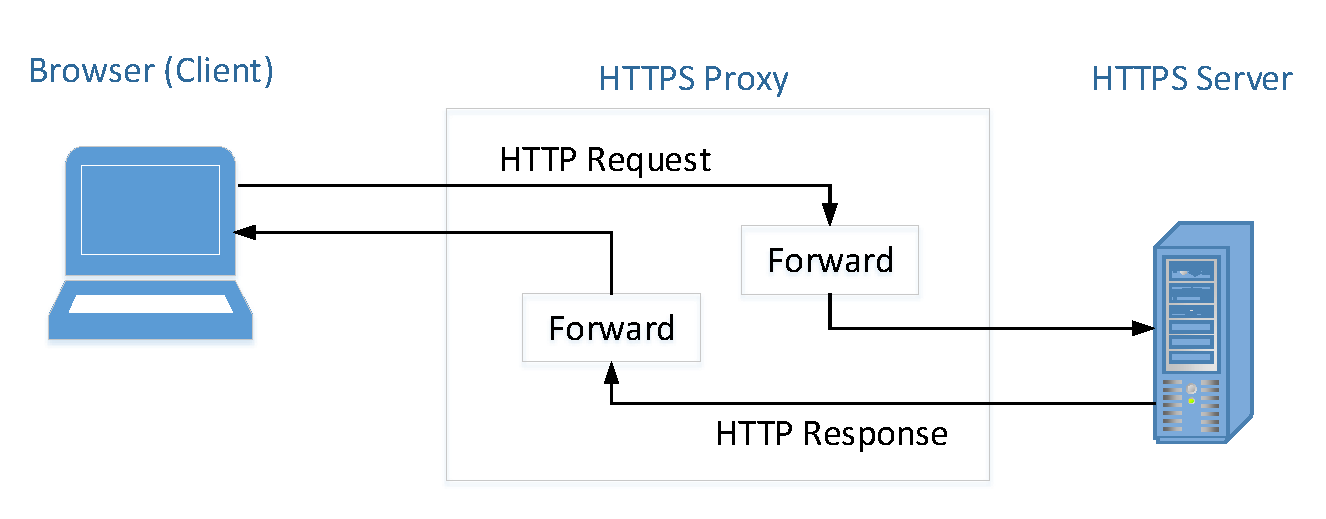
\includegraphics[width=0.8\textwidth]{\tlsFigs/httpsproxy.pdf}
\caption{How \texttt{mHTTPSproxy} works}
\label{tls:fig:proxy}
\end{figure}

代理实际上是 TLS 客户端和服务器程序的组合。
对于浏览器, TLS 代理只是一个服务器程序,
它从浏览器(客户端)获取 HTTP 请求,并向其返回 HTTP 响应。
代理本身不会生成任何 HTTP 响应,
而是将 HTTP 请求转发到实际的 Web 服务器,然后从 Web 服务器获取 HTTP 响应。
对于实际的 Web 服务器, TLS 代理只是一个客户端程序。
收到响应后,代理将响应转发给浏览器,即真正的客户端。
因此,通过集成在前两个任务中实现的客户端和服务器程序,学生应该能够实现基本的代理工作。

应该注意的是,此任务的目的是使用简单的代理来了解当 PKI 基础结构受到威胁时,
中间人攻击如何工作。
并不是要实现商业化的 HTTPS 代理,因为要使代理在每个 Web 服务器上都工作并不容易,
需要考虑 HTTP 协议的许多方面。
由于本实验的重点是 TLS ,因此学生可以选择两个不同的服务器,并演示其代理服务器可用于这些服务器。
对商业化的 HTTPS 代理感兴趣的学生从网络上寻找其他资料,例如开源 \texttt{mitmproxy} 。


\paragraph{处理多个 HTTP 请求}
浏览器可能会同时向服务器发送多个 HTTP 请求,因此在从浏览器接收到 HTTP 请求之后,
最好生成一个线程来处理该请求,以便代理程序可以处理多个同时请求。
以下代码段显示了如何创建一个新的线程来处理每个 TLS 连接。

\begin{lstlisting}
import threading

while True:
    sock_for_browser, fromaddr = sock_listen.accept()
    ssock_for_browser = context_srv.wrap_socket(sock_for_browser,
                                                server_side=True)
    x = threading.Thread(target=process_request, args=(ssock_for_browser,))
    x.start()
\end{lstlisting}


该线程将执行 \texttt{process\_request} 函数中的代码,
该函数将 HTTP 请求从浏览器转发到服务器,然后将 HTTP 响应从服务器转发到浏览器。
以下提供了代码框架:


\begin{lstlisting}
def process_request(ssock_for_browser):
    hostname = 'www.example.com'

    # Make a connection to the real server
    sock_for_server  = socket.create_connection((hostname, 443))
    ssock_for_server = ... # [Code omitted]: Wrap the socket using TLS

    request = ssock_for_browser.recv(2048)

    if request:
        # Forward request to server
        ssock_for_server.sendall(request)

        # Get response from server, and forward it to browser
        response = ssock_for_server.recv(2048)
        while response:
            ssock_for_browser.sendall(response) # Forward to browser
            response = ssock_for_server.recv(2048)

    ssock_for_browser.shutdown(socket.SHUT_RDWR)
    ssock_for_browser.close()
\end{lstlisting}


\paragraph{客户端设置}
对于此任务,由于我们将使用浏览器,因此将使用虚拟机作为客户端或者受害者,而不是使用 client 容器。
在实际攻击中,当受害者尝试访问 Web 服务器(例如 \url{www.example.com} )时,
我们将发起攻击将受害者重定向到我们的代理。
这通常通过 DNS 攻击, BGP 攻击或其他重定向攻击来完成。
但事实上我们不会进行此类攻击。
我们只需将以下条目添加到主机 VM 上的 \texttt{/etc/hosts} 文件中
( \texttt{10.9.0.143} 是 mitm-proxy 容器的 IP 地址)。

\begin{lstlisting}
10.9.0.143   www.example.com
\end{lstlisting}

通过执行上述操作,我们模拟了重定向攻击的结果:
受害者到 \url{www.example.com} 的流量将被重定向到攻击者机器上,
你的 \texttt{mHTTPSproxy} 在那里等待 HTTP 请求。


\paragraph{任务}
学生应该实现简单的 \texttt{mHTTPSproxy},并在代理容器上运行它。
在此 MITM 攻击中,我们假设攻击者已经破坏了受信任的 CA ,
并且能够使用 CA 的私钥为任何域名生成伪造但有效的证书。
在本实验中,浏览器已信任任务 2 中生成的 CA 证书,并且我们假定此 CA 的私钥已被破坏,
因此你(攻击者)可以使用它为任何 Web 服务器伪造证书。
请在以下情况下展示您的 MITM 攻击:


\begin{itemize}
    \item 针对你自己的服务器发起中间人攻击。

    \item 在真实的 HTTPS 网站上发起 MITM 攻击。
          你可以选择一个网站,找到一个需要登录的帐户,然后使用你的 MITM 代理窃取密码。
          许多流行的服务器(例如 Facebook )具有复杂的登录机制,
          你可以找一个具有简单登录机制的服务器。
          如果你使用的是真实密码,请记住在实验报告中隐藏密码。
\end{itemize}



\paragraph{清理} 完成此任务后,请记得从浏览器中删除 CA 的证书,
并且删除在虚拟机上添加到 \texttt{/etc/hosts} 的所有条目。



% *******************************************
% SECTION
% *******************************************
\section{Submission}

%%%%%%%%%%%%%%%%%%%%%%%%%%%%%%%%%%%%%%%%

You need to submit a detailed lab report, with screenshots,
to describe what you have done and what you have observed.
You also need to provide explanation
to the observations that are interesting or surprising.
Please also list the important code snippets followed by
explanation. Simply attaching code without any explanation will not
receive credits.

%%%%%%%%%%%%%%%%%%%%%%%%%%%%%%%%%%%%%%%%

\end{document}







